\chapter{Baggrund}
\section{Kroppens kredsløb}
Det menneskelige kredsløb har til hovedfunktion at transportere de forskellig livsnødvendige stoffer rundt i kroppen. Kredsløbet transporter også kroppens affaldsstoffer ud til de organer, hvor de kan udskilles. Kredsløbet er altså kroppens transportmiddel. 
\\ \\
Kredsløbet består af hjertet samt et system af blodkar. Hjertet er opdelt i to halvdele, som begge fungere som en pumpe. Den højre side af hjertet pumper blodet gennem det lille kredsløb (lungekredsløb), mens venstre side pumper blodet gennem det store kredsløb (legemskredsløbet). 

\begin{figure}[H]
	\centering
	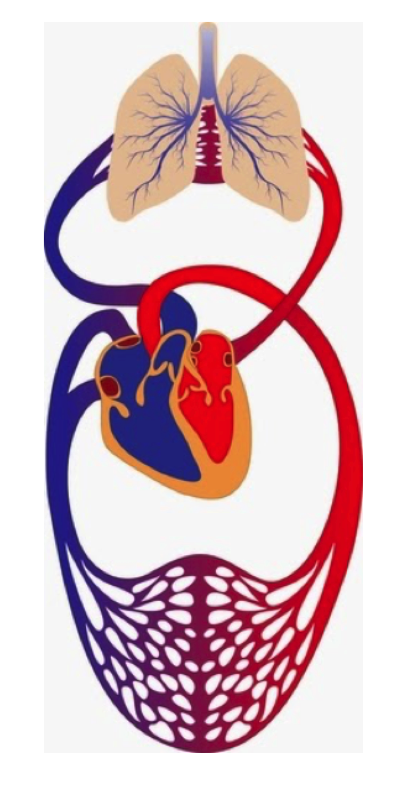
\includegraphics[width=0.4\textwidth]{Figurer/Snip20151209_69}
	\caption{Illustration af kroppens kredsløb}
\end{figure}

På Figur 3.1 ses det lille- og det store kredsløb. Hjertet er placeret i midten, hvor det er delt op i højre- og venstre side. Højre atrium modtager iltfattigt veneblod, som har været igennem det store kredsløb. Fra atrium strømmer blodet til højre ventrikel, som pumper det gennem lungearterien til lungerne, hvor blodet får tilført ilt og afgiver kuldioxid. Blodet skal nu retur til hjertet gennem lungerne til venstre atrium. Fra venstre atrium strømmet blodet til venstre ventrikel, hvor det efterfølgende pumpes ud gennem aorta til alle kroppens organer, som har brug for ilt. Blodet bliver igen iltfattigt og skal tilbage til højre side af hjertet, før det kan benyttes igen. Mennesket har ca. 5 liter blod i kroppen, som bliver genbrugt igen og igen. Den menneskelig krop kan prioritere det iltrige blod i forhold til, hvor der er mest brug for det. 
\\ \\
Systemet af blodkar består af tre forskellige typer. Arterier, vener og kapillærer. Arterieren leder blodet fra ventrikler til kroppens organer, venerne sørger for for returnering af langt det meste til atrierne, og kapillærerne forbinder arterier og vener. 
 \\
Arterierne er som sagt de blodkar, der modtager blodet fra hjertet. Disse skal være elastiske, da de udsættes for et stort tryk, når hjertet trækker sig sammen og pumper blodet ud i det store kredsløb. Arterierne forgrener sig til arterioler, der igen forgrener sig kapillærer. Det er i disse blodkar udvekslingen af næringsstoffer, luftarter og affaldsstoffer til cellerne sker. Venolerne samler blodet fra kapillærerne og fører det over i venerne, som returnerer det til hjertets højre side.
\\ \\
Hjertet har i alt fire hjerteklapper. To af klapperne betegnes som AV-klapperne (Atrioventrikulærklapperne). Disse adskiller atrium og ventrikel i henholdsvis højre- og venstre side. Den i højre side kaldes tricuspidalklappen, mens den i venstre side kaldes bicuspidalklappen. Den tredje kaldes pulmonalklappen og sidder mellem lungearterien og højre atrium. Den fjerde kaldes aortaklappen og sidder mellem aorta og venstre ventrikel. Alle hjerteklapperne er designet således, at blodet kun kan løbe den ene vej igennem disse. Åbningen og lukningen af disse er en passiv proces, som bestemmes af forskelle i væsketrykket på de to sider af klapperne. 

\begin{figure}[H]
	\centering
	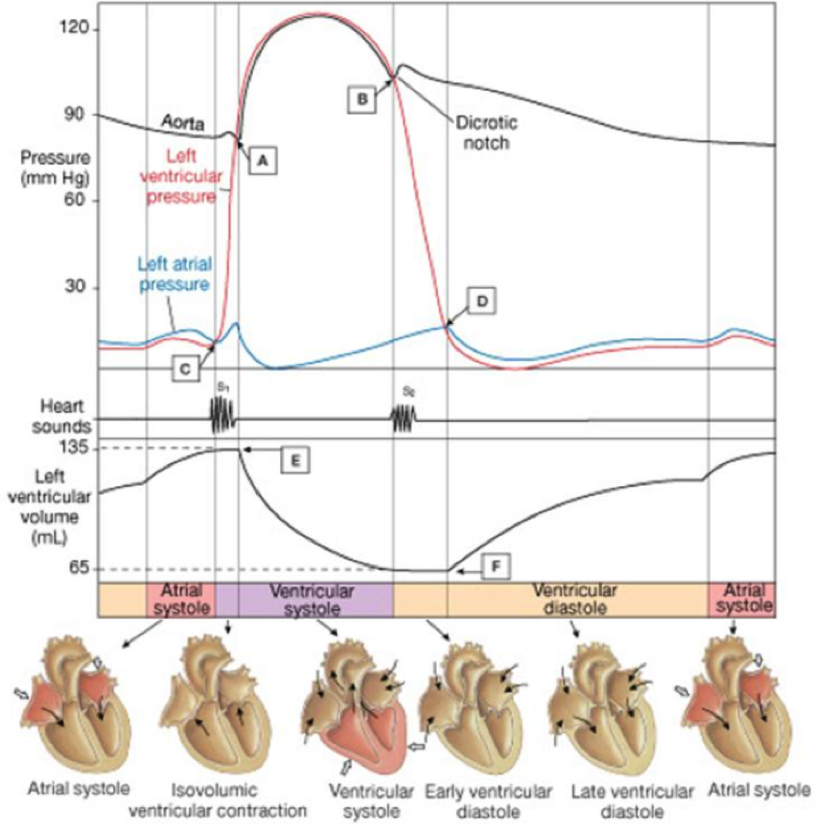
\includegraphics[width=0.8\textwidth]{Figurer/Snip20151209_68}
	\caption{Illustration af hjertet cyklus}
\end{figure}

På Figur 3.2 illustreres hjertets cyklus ud fra trykket (mmHg) i henholdsvis venstre atrium og ventrikel, hjertelyde, lukning og åbning af hjerteklapperne samt volumen i venstre ventrikel. Der er i alt illustreret fem faser for hjertet. \\
Den første fase kaldes atrium systole. Her er trykket højere i atrium end i ventrikel og dermed er bicuspidalklappen åben, så blodet kan strømme fra atrium til ventrikel. Det ses også at volumen i ventriklen stiger. \\
Når trykket i ventriklen overstiger trykket i atrium lukker bicuspidalklappen og første hjertelyd forekommer på grund af vibrationer, befinder hjertet sig i anden fase. Her stiger trykket i atrium kort og lidt, mens trykket i ventriklen stiger voldsomt. Det ses at volumen forbliver konstant i denne fase. \\
I tredje fase over stiger trykket i ventriklen trykket i aorta og aortaklappen åbner sig – denne fase kaldes ventrikel systole. Volumen i ventriklen falder i takt med at ventriklerne trækker sig sammen. Det ses at i denne fase følger trykket i ventriklen og aorta hinanden. Forklaringen på dette er, at aorta har en høj compliance, som gør at den kan udvide sig og på den måde opretholde trykket. Samtidigt modtager atrium blod fra lungevenerne, hvilket gør at trykket i atrium stiger. \\
Fjerde fase forekommer, når trykket i ventriklen er under trykket i aorta igen, hvilket forårsager, at aortaklappen lukkes igen og anden hjertelyd kan høres. Denne fase kaldes tidlig ventrikel diastole. Her begynder ventriklen at slappe af. \\
Femte fase begynder, når ventrikel slapper så meget af, at trykket kommer under trykket i atrium. Her åbner bicuspidalklappen igen og fyldningen af ventriklen begynder stille og rolig igen. Det ses at volumen langsomt stiger. Denne fase kaldes sen ventrikel diastole. Efter denne fase begynder første fase igen, hvor trykket i atrium stadigvæk er større end i ventriklen. 
\\\\
Væskestrømningen er det væskevolumen, der fragtes gennem et rør pr. tidsenhed. Væskestrømningen, Q, stiger med trykforskellen i begyndelsen og slutning af røret, $\Delta$P, samt aftager med rørets modstand mod væskestrømmen, R: 

\begin{equation}
Q = \frac{\Delta P}{R}
\end{equation}

Trykforskellen udgør drivkraften for væskestrømmen gennem røret. Denne strøm går fra højt til lavt tryk, hvilket hjertets kontraktion fremkalder. Modstanden i røret er et udtryk for gnidningsmodstanden mellem den væske, der bevæger sig og rørvæggen, som er i ro. Denne modstand har indflydelse på væskestrømmen i et rør. Efterhånden som væsken strømmer gennem røret, falder trykket i væsken. Ved stigende modstand mod væskestrømmen, stiger dette trykfald. Når modstand mod væskestrømmen i røret stiger, bliver væskestrømmen mindre under forudsætning af, at trykforskellen ikke stiger tilsvarende. Denne modstand bestemmes af tre faktorer: rørets længde, indre diameter og væskens viskositet. 
Modstanden stiger med øget rørlængde, reduceret diameter og øget viskositet. 
\\ \\
Væskestrømmen i blodkar kaldes blodstrømmen. Hjertets kontraktion sætter væsken i rørene under tryk – jo kraftigere hjertet pumper, jo større bliver trykforskellen og dermed blodstrømningen. Diameteren af blodkarret har stor betydning for modstanden mod blodstrømmen. Modstanden er mindre, og blodstrømmen er større i de store kar end i de små.
\\\\
Når blodet går fra hjertet til kapillærerne forgrener blodkarrene sig til mange små og smallere kar. Herved stiger det samlede tværsnitsareal kraftigt, og der sker automatisk en aftagning af blodets strømningshastighed. Blodets lave strømningshastighed i kapillærerne er vigtig for stofudvekslingen, der sker gennem kapillærvæggene. Ved blodets vej tilbage fra kapillærerne til hjertet stiger strømningshastigheden igen, idet det samlede tværsnitsareal aftager.
\\\\
Væskestrømmens tryk gennem et rør er som nævnt trykforskellen mellem rørets begyndelse og slutning. I det store kredsløb er trykket lig med forskellen mellem trykket i aorta og trykket i højre atrium. Det tryk, der er i højre atrium, er ved normale tilstande meget tæt på nul, og derved kan man betragte det gennemsnitlige tryk i aorta som trykforskellen. Det arterielle blodtryk er det tryk, der er i de store arterier, som er ligeså højt som trykket i aorta. Modstanden i hele det store kredsløb kaldes den totale perifere modstand. Formlen for sammenhængen mellem væskestrøm, tykforskel og modstand kan også overføres til det store kredsløb, hvor minutvolumen, MV, stiger med blodtrykket, BT, og aftager med den totale perifere modtand, TPM:

\begin{equation}
\centering
MV = \frac{BT}{TPM}
\end{equation}

Dette betyder, at ændringerne i det arterielle blodtryk skyldes forandringer i enten hjertets minutvolumen eller blodkarrenes modstand mod væskestrømmen. 
Arteriosklerose ændres modstanden i blodkarrene, da der sker en indsnævring af arterierne og arteriolerne. Dette medfører en belastning for hjertet, da den samme mængde blod ønskes transporteres rundt i kroppen på samme tid, da man gerne vil opretholde minutvolumen. Hvis denne sygdom ikke behandles vil indsnævringen blive så slem, at minutvolumen ikke heller kan opretholdes, og patienten vil nu være i en livstruende sygdom. Patientens arterielle blodtryk vil stige i takt med indsnævringen. 
\\\\
Det arterielle blodtryk (systole og diastole) fortæller altså noget om, hvordan hjerte arbejder. Hvis man har et arterielt blodtryk, hvor systole er over 140 og diastole er over 90, siger man, at man har et forhøjet blodtryk. Et forhøjet blodtryk kan have anledning til forskellige sygdomme, f.eks. arteriosklerose. 
\\\\
Der findes flere forskellige metoder til at måle blodtryk – både invasivt og ikke-invasivt. I begge tilfælde bestemmes en værdi for det systoliske- og det diastoliske blodtryk. Non-invasivt kan blodtrykket måles med ultralyd eller ved den oscillometriske metode med manchet, stetoskop og kviksølvsmanometer. Derudover findes der også den automatiserede teknik, der erstatter stetoskopet med en mikrofon.
\\\\
I dette projekt er der blevet designet et monitoreringssystem til at vise en invasiv blodtryksmåling.  



\section{Invasiv blodtryksmåling}
Invasive blodtryksmålinger bruges ofte til monitorering af hæmodynamiske data, og anvendes som regel hos svært syge patienter på eksempelvis intensiv afdeling, samt ved større operationer. Ved den invasive blodtryksmåling måles blodtrykket via et kateter, der lægges ind i arterien. Med denne metode får man et mere præcist og kontinuerligt billede af, hvordan hjertet arbejder. 

\begin{figure}[H]
	\centering
	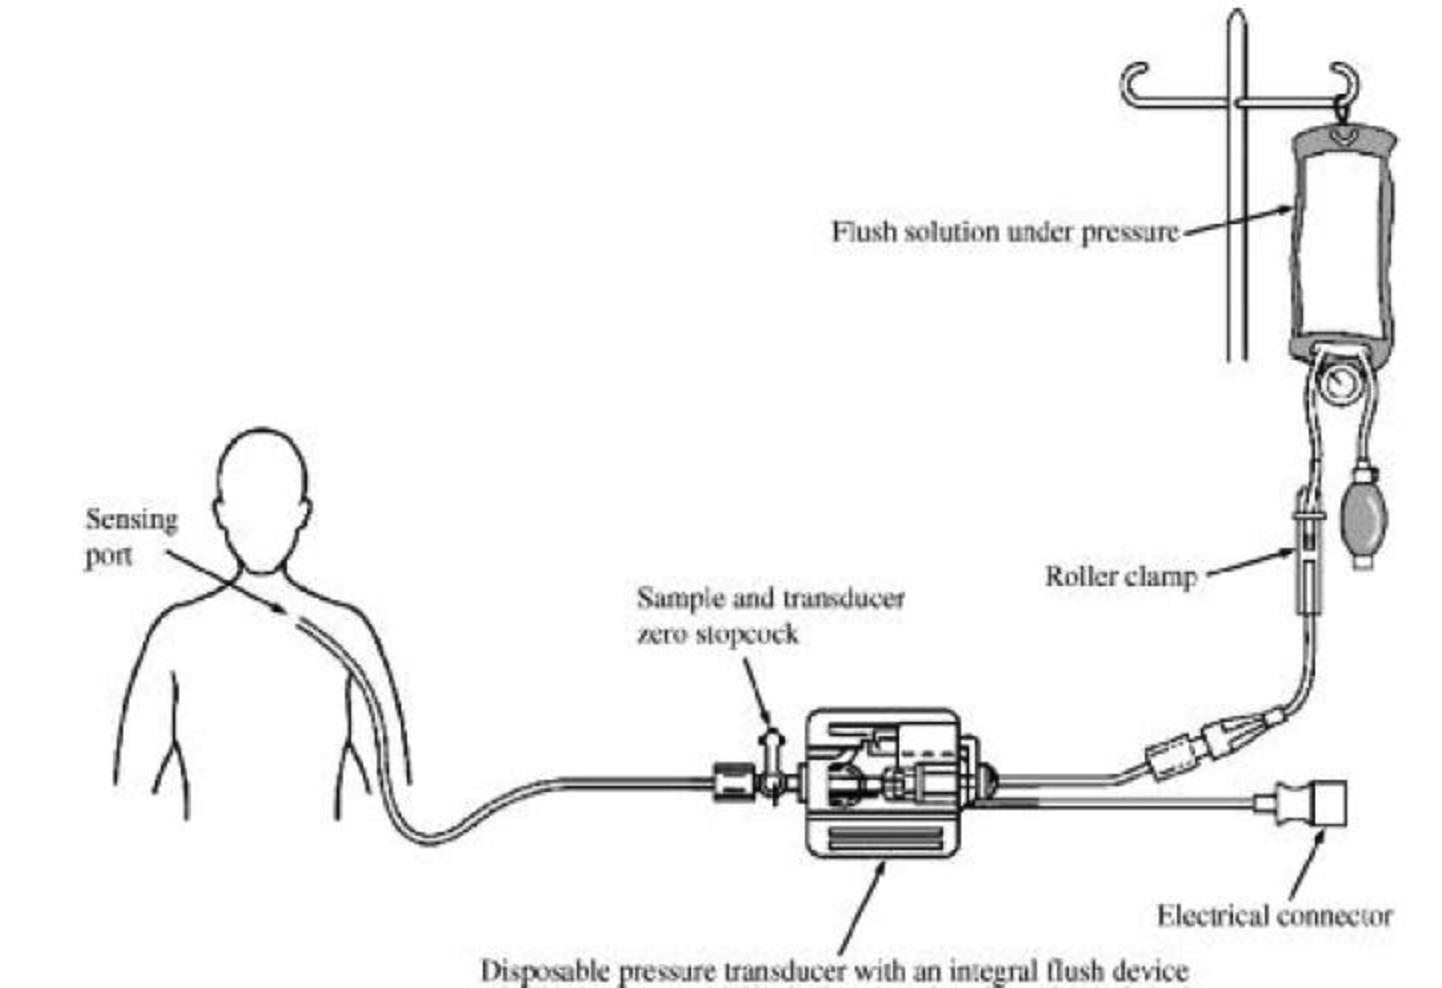
\includegraphics[width=1\textwidth]{Figurer/Snip20151207_50}
	\caption{Måleopstilling}
\end{figure}

På Figur 3.3 ses måleopstillingen for den invasive blodtryksmåling. Der føres et væskefyldt kateter ind i personens arterie. Trykposen på Figur 3.1 er fyldt med natriumklorid og fungerer som en del af flushmekanismen, som benyttes til at fjerne bobler fra det væskefyldte kateter. Trykket i posen pumpes op til mellem 180 til 300 mmHg, hvilket er over det systoliske blodtryk. \\
Slangen fra trykposen går ned til tryktransduceren og flushsystemet. Når fluchsystemet startes, vil man på monitoren kunne se, at trykket stiger til det tryk, der er i trykposen. Når dette stoppes, er systemet udviklet således, at der altid vil løbe en dråbe natriumklorid ind i kateteret. Dette forhindrer blod i at strømme ud i kateteret. Trykket i det væskefyldte kateter er lig med trykket i personens arterie. Det er dette tryk, som tryktransduceren transformerer om til et elektrisk signal, som kontinuert vises på monitoren. \\
Tryktransduceren består af fire strain gauges, også kaldet en wheatstone bro. Strain gauges er en modstandståd, der kan foldes og limes på et hvilket som helst materiale. Modstanden, R bestemmes ud fra længden, l, resistiviteten, $\varrho$ og tværsnitsarealet, A. 

\begin{equation}
	R = \frac{l \cdot \varrho}{A}
\end{equation}

Ændres en eller flere af disse, vil modstandsværdien ændres efterfølgende. Materialet, som strain gauges er limet fast på, kan ændre form, hvilket strain gauges registrerer. Det er dette, tryktransduceren benytter sig af. De fire strain gauges er limet fast på en membran, som sidder for enden af det væskefyldte kateter. Når blodtrykket ændrer sig, påvirkes membranen, da den har en meget højere compliance end selve det væskefyldte kateter. Denne forskel i compliance er en af grundene til, at dette system kan registre selv de mindste trykændringer. \\ 
Trykændringer registreres af de fire strain gauges, som transformerer dem om til det elektriske signal, hvilket afbildes grafisk. På figur 3.4 ses afbildningen af en invasiv blodtryksmåling, hvor det også er muligt at aflæse det diastoliske og systoliske blodtryk.  Det diastoliske tryk svarer til minimumspunkterne, hvor toppunkterne svarer til det systoliske tryk.


\begin{figure}[H]
	\centering
	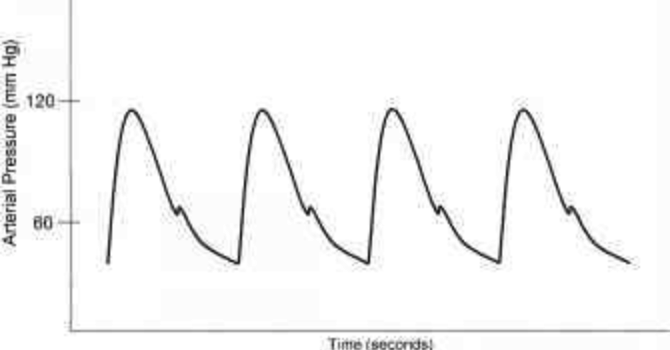
\includegraphics[width=1\textwidth]{Figurer/Snip20151207_51}
	\caption{Grafisk afbildning af en invasiv blodtryksmåling}
\end{figure}

Strain gauges benyttes i dette tilfælde, da man ønsker, at selv den mindste trykændring skal kunne registreres. Da disse modstandsændringer er så små, ønskes disse forstærkes op. For at kunne gøre dette bedst muligt, skal der benyttes et måle setup, som er centraliseret omkring nul. Til dette bruges en Wheatstone bro, nærmere en helbro, se Figur 3.5. 

\begin{figure}[H]
	\centering
	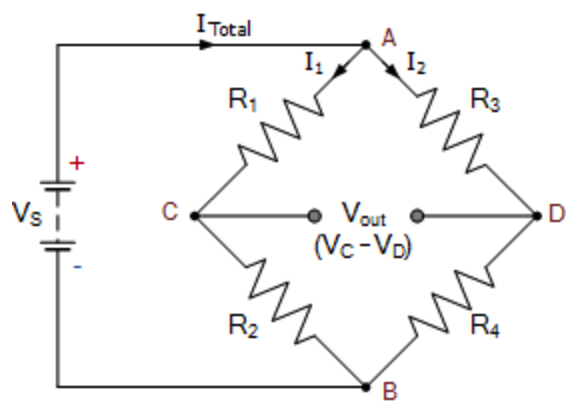
\includegraphics[width=0.5\textwidth]{Figurer/Snip20151207_63}
	\caption{Wheatstone bro}
\end{figure}

En Wheatstone bro er et kredsløb, der består af to serieforbindelser af to modstande, som sidder i parallelforbindelse. I mellem serieforbindelserne kan $V_{out}$ beregnes ud fra spændingen ved punkt C og punkt D.

\begin{equation}
	V_{out} = V_{C} - V_{D}
\end{equation} 

Hvis modstandene $R_{1}$ og $R_{3}$ samt $R_{2}$ og $R_{4}$ er ens, vil $V_{out}$ være lig med nul og broen vil være i balance, se Figur 3.6. 

\begin{figure}[H]
	\centering
	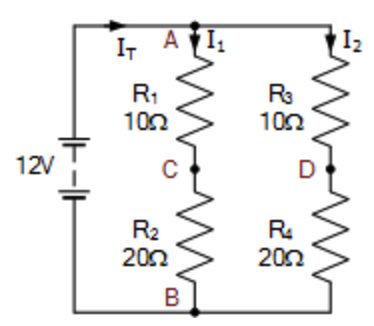
\includegraphics[width=0.5\textwidth]{Figurer/Snip20151207_64}
	\caption{Wheatstone bro i balance}
\end{figure}

Hvis modstandene $R_{1}$ og $R_{3}$ samt $R_{2}$ og $R_{4}$ er forskellige af hinanden, vil $V_{out}$ være forskellig fra nul og broen vil være i ubalance, se Figur 3.7. 

\begin{figure}[H]
	\centering
	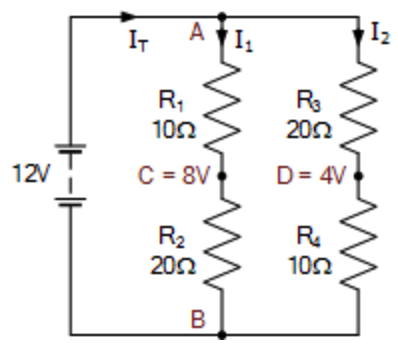
\includegraphics[width=0.5\textwidth]{Figurer/Snip20151207_65}
	\caption{Wheatstone bro i ubalance}
\end{figure}

Når trykændringerne påvirker membranen, vil de fire strain gauges ændre form og dermed ændre modstandsværdi. Dette skaber ubalance i Wheatestone broen, og spændingen ændrer sig i takt med dette. Spændingsændringen kan beregnes ud fra fomlen (3.5).


\begin{equation}
\centering
\frac{v_{0}}{v_{in}} = \frac{\Delta R}{R}
\end{equation}


\subsection{Dynamiske egenskaber}
Et væskefyldt kateter har inerti, friktion og elastiske egenskaber, der også kan betegnes som inertans, modstand og compliance (eftergivelighed). Disse egenskaber kan beskrives som elektriske komponenter i form af en induktor, resistor og kapacitor, se Figur 3.8.

\begin{figure}[H]
	\centering
	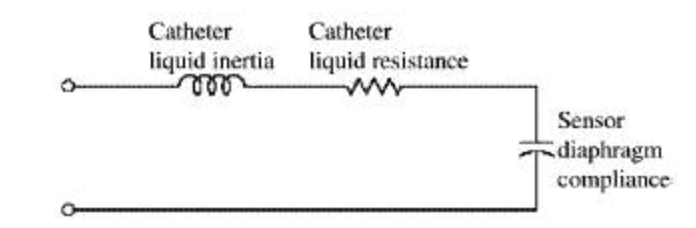
\includegraphics[width=1\textwidth]{Figurer/Snip20151207_58}
	\caption{Anden ordens lavpassystem}
\end{figure}

De forskellige egenskaber kan udtrykkes ved ligninger (3.6), (3.7) og (3.8). 

\begin{equation}
\centering
L = \frac{l\cdot p}{\pi\cdot r^2}
\end{equation}

\begin{equation}
\centering
R = \frac{8\cdot \mu\cdot l}{\pi\cdot r^4}
\end{equation}

\begin{equation}
C = \frac{\Delta V}{\Delta P} = \frac{1}{E_{d}}
\end{equation}

Figur 3.8 viser et anden ordens lavpassystem, der kan beskrives med følgende to overføringsfunktioner:

\begin{equation}
T(s) = \frac{K s}{s^2 + 2\cdot \zeta\cdot \omega_{0}\cdot s + \omega_{0}^2}
\end{equation}

\begin{equation}
T(s) = \frac{k}{s^2 + \frac{\omega_{0}}{Q} \cdot s + \omega_{0}^2}
\end{equation}

Ud fra disse overføringsfunktioner kan knækfrekvensen, $f_{0}$ og flowet, Q findes:

\begin{equation}
f_{0} = \frac{r}{2} \cdot \sqrt{\frac{1}{l\cdot p \cdot \pi}\cdot \frac{\Delta P}{\Delta V}}
\end{equation}

\begin{equation}
Q = \frac{r^3}{8 \cdot \mu} \cdot \sqrt{\frac{\rho \cdot \pi}{l}\cdot \frac{\Delta P}{\Delta V}}
\end{equation}
 \\
 
Figur 3.9 viser et bodeplot for amplitude og fasen for lavpasfilteret.

\begin{figure}[H]
	\centering
	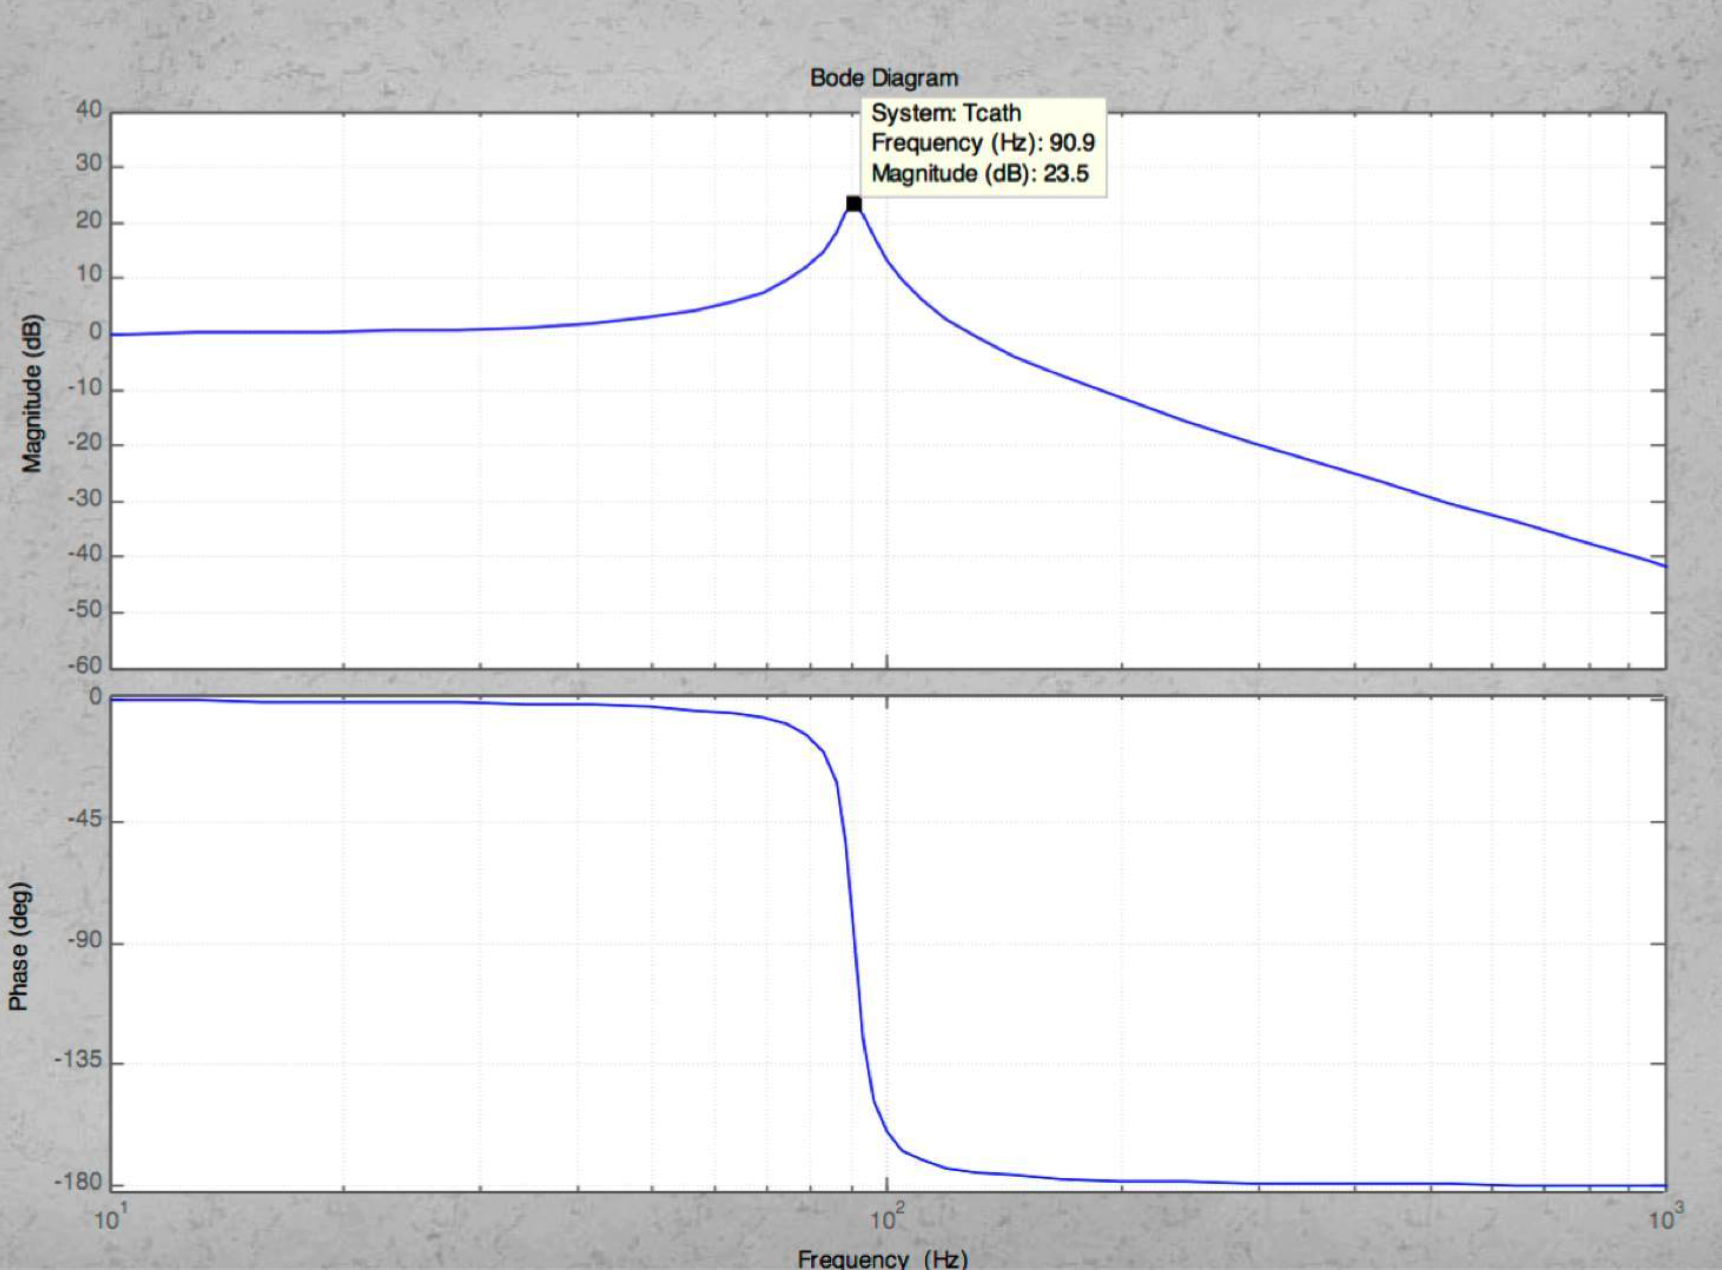
\includegraphics[width=0.8\textwidth]{Figurer/Snip20151207_61}
	\caption{Bodeplot}
\end{figure}

Det interessante er, at knækfrekvensen ligger ved 90 Hz. Dette betyder, at systemet medtager frekvenser op til de 90 Hz, hvilket er mere end, hvad systemet skal kunne klare ift. en blodtryksmåling, hvis frekvenser ikke kommer over 50 Hz.
\\\\ 

På figur 3.10 kan man se, hvorledes bobler i systemet påvirker systemets knækfrekvens og dermed dens båndbredde samt dæmpningsfaktoren.   

\begin{figure}[H]
	\centering
	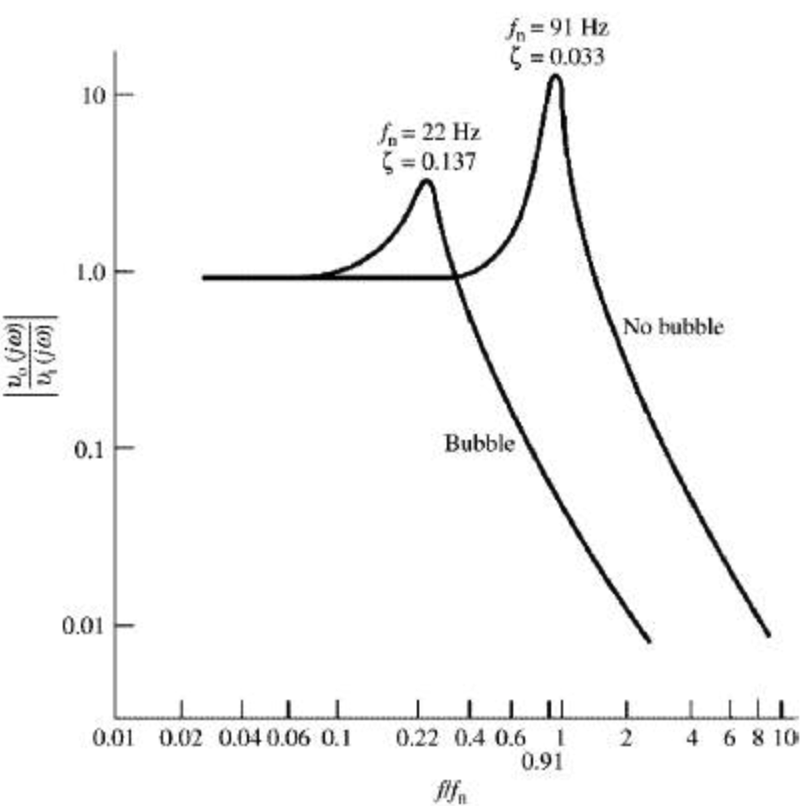
\includegraphics[width=0.5\textwidth]{Figurer/Snip20151207_62}
	\caption{Diagram over knækfrekvensen og dæmpningsfaktoren påvirket af bobler og uden}
\end{figure}

Hvis der er bobler tilstede i kateteret, bliver der samtidig tilført ekstra compliance. Dette medvirker til, at knækfrekvensen forekommer tidligere, hvilket betyder, at båndbredden bliver mindre. Som det ses i Figur 3.10 er knækfrekvensen mindre og dæmpningsfaktoren større, når der er bobler tilstede i kateteret.\\ 
En mindre knækfrekvens forårsager, at systemet kun lukker frekvenser fra 0 til 22 Hz igennem, hvilket ikke er tilstrækkeligt til at repræsentere en optimal blodtryksmåling. Dæmpningsfaktoren øges, når compliance stiger. Det vil sige, at jo større dæmpningsfaktor og compliance, jo mindre quality, jo større tab over system. Det ses ved ligningen for dæmpningsfaktoren:

\begin{equation}
\centering
\zeta = \frac{1}{2 \cdot Q}
\end{equation}

For at undgå bobler i væsken, kan man benytte føromtalte flushmekanisme, hvor man vha. trykposen kan erstatte luftbobler med natriumklorid.














